\def\year{2020}\relax
%File: formatting-instruction.tex
\documentclass[letterpaper]{article} % DO NOT CHANGE THIS
\usepackage{aaai20}  % DO NOT CHANGE THIS
\usepackage{times}  % DO NOT CHANGE THIS
\usepackage{helvet} % DO NOT CHANGE THIS
\usepackage{courier}  % DO NOT CHANGE THIS
\usepackage[hyphens]{url}  % DO NOT CHANGE THIS
\usepackage{graphicx} % DO NOT CHANGE THIS
\urlstyle{rm} % DO NOT CHANGE THIS
\def\UrlFont{\rm}  % DO NOT CHANGE THIS
\usepackage{graphicx}  % DO NOT CHANGE THIS
\frenchspacing  % DO NOT CHANGE THIS
\setlength{\pdfpagewidth}{8.5in}  % DO NOT CHANGE THIS
\setlength{\pdfpageheight}{11in}  % DO NOT CHANGE THIS
\usepackage{bm}
\usepackage{amsfonts}
\usepackage{amsmath}
\usepackage{multirow}
\usepackage{color}

\newcommand{\cxj}[1]{\textcolor{red}{(#1)}}
\newcommand{\rpl}[1]{\textcolor{yellow}{(#1)}}
\newcommand{\mdf}[1]{\textcolor{blue}{#1}}
\newcommand{\vset}[1]{#1_{1:T}} %% denote for the input frames 
\newcommand{\msset}[1]{\{#1_{t-7},#1_{t-3},#1_{t},#1_{t+3},#1_{t+7}\}}
\newcommand{\gtframe}{\widetilde{Y}_t} %% denote for the ground truthe frame Y_t 

%\nocopyright
%PDF Info Is REQUIRED.
% For /Author, add all authors within the parentheses, separated by commas. No accents or commands.
% For /Title, add Title in Mixed Case. No accents or commands. Retain the parentheses.
 \pdfinfo{
/Title (Spatio-Temporal Structure Enhancement for video inpainting)
/Author (Anomymous sumbission)
} %Leave this	
% /Title ()
% Put your actual complete title (no codes, scripts, shortcuts, or LaTeX commands) within the parentheses in mixed case
% Leave the space between \Title and the beginning parenthesis alone
% /Author ()
% Put your actual complete list of authors (no codes, scripts, shortcuts, or LaTeX commands) within the parentheses in mixed case. 
% Each author should be only by a comma. If the name contains accents, remove them. If there are any LaTeX commands, 
% remove them. 

% DISALLOWED PACKAGES
% \usepackage{authblk} -- This package is specifically forbidden
% \usepackage{balance} -- This package is specifically forbidden
% \usepackage{caption} -- This package is specifically forbidden
% \usepackage{color (if used in text)
% \usepackage{CJK} -- This package is specifically forbidden
% \usepackage{float} -- This package is specifically forbidden
% \usepackage{flushend} -- This package is specifically forbidden
% \usepackage{fontenc} -- This package is specifically forbidden
% \usepackage{fullpage} -- This package is specifically forbidden
% \usepackage{geometry} -- This package is specifically forbidden
% \usepackage{grffile} -- This package is specifically forbidden
% \usepackage{hyperref} -- This package is specifically forbidden
% \usepackage{navigator} -- This package is specifically forbidden
% (or any other package that embeds links such as navigator or hyperref)
% \indentfirst} -- This package is specifically forbidden
% \layout} -- This package is specifically forbidden
% \multicol} -- This package is specifically forbidden
% \nameref} -- This package is specifically forbidden
% \natbib} -- This package is specifically forbidden -- use the following workaround:
% \usepackage{savetrees} -- This package is specifically forbidden
% \usepackage{setspace} -- This package is specifically forbidden
% \usepackage{stfloats} -- This package is specifically forbidden
% \usepackage{tabu} -- This package is specifically forbidden
% \usepackage{titlesec} -- This package is specifically forbidden
% \usepackage{tocbibind} -- This package is specifically forbidden
% \usepackage{ulem} -- This package is specifically forbidden
% \usepackage{wrapfig} -- This package is specifically forbidden
% DISALLOWED COMMANDS
% \nocopyright -- Your paper will not be published if you use this command
% \addtolength -- This command may not be used
% \balance -- This command may not be used
% \baselinestretch -- Your paper will not be published if you use this command
% \clearpage -- No page breaks of any kind may be used for the final version of your paper
% \columnsep -- This command may not be used
% \newpage -- No page breaks of any kind may be used for the final version of your paper
% \pagebreak -- No page breaks of any kind may be used for the final version of your paperr
% \pagestyle -- This command may not be used
% \tiny -- This is not an acceptable font size.
% \vspace{- -- No negative value may be used in proximity of a caption, figure, table, section, subsection, subsubsection, or reference
% \vskip{- -- No negative value may be used to alter spacing above or below a caption, figure, table, section, subsection, subsubsection, or reference


\setcounter{secnumdepth}{0} %May be changed to 1 or 2 if section numbers are desired.

% The file aaai20.sty is the style file for AAAI Press 
% proceedings, working notes, and technical reports.
%
\setlength\titlebox{2.5in} % If your paper contains an overfull \vbox too high warning at the beginning of the document, use this
% command to correct it. You may not alter the value below 2.5 in
\title{Spatio-Temporal Structure Enhancement for video inpainting}
%Your title must be in mixed case, not sentence case. 
% That means all verbs (including short verbs like be, is, using,and go), 
% nouns, adverbs, adjectives should be capitalized, including both words in hyphenated terms, while
% articles, conjunctions, and prepositions are lower case unless they
% directly follow a colon or long dash
\author{Anonymous submission}
 \begin{document}

\maketitle

\begin{abstract}
	Video inpainting targets to fill the missing regions in videos, which requires high spatio-temporal consistency.
	However, recent deep-learning based methods focus on temporally smoothening inpainted frames via motion information, but the detailed structure clues are much less explored.
	In this paper, we propose a novel Spatio-temporal Structure Enhancement Network (SSENet) for structure-preserved video inpainting. 
	Specifically, SSENet first synthesizes the edge information across frames, based on an encoder-decoder with heterogeneous receptive field. Then, a coarse-to-fine adversarial model is designed for frame inpainting.
	Explicitly, a structure attention module is developed to extract the spatial correlation between video contents and completed edge. This can facilitate the structure-enhanced video inpainting.  
	Meanwhile, the missing flow is also predicted to ensure the temporal consistency of both edge and video frames, via flow-guided warping and temporal ensemble.  
	Consequently, the inpainted frames by SSENet are visually pleasing in detailed structures and temporally stabilized, with low time cost. 
	Experiments on YouTubeVOS and DAVIS show that SSENet obtains state-of-the-art performance and few artifacts, which demonstrate the significance of structure enhancement in video inpainting.
	
\end{abstract}


 


\section{Introduction}


Video inpainting aims to recover the missing contents of given videos, which can assist lots of practical applications, e.g., video restoration and augmented reality. Compared with image inpainting, video inpainting is much more challenging due to the extra time dimension. It requires not only reasonable spatial structures but also temporal consistency. 
Though great progress has been made in 2D image inpainting using deep learning techniques \cite{yu2018free,Xiong_2019_CVPR}, directly applying these approaches to each individual frame in video inpainting could lead to artifacts, flickers and jitters. 

\begin{figure}[t]
	\centering
	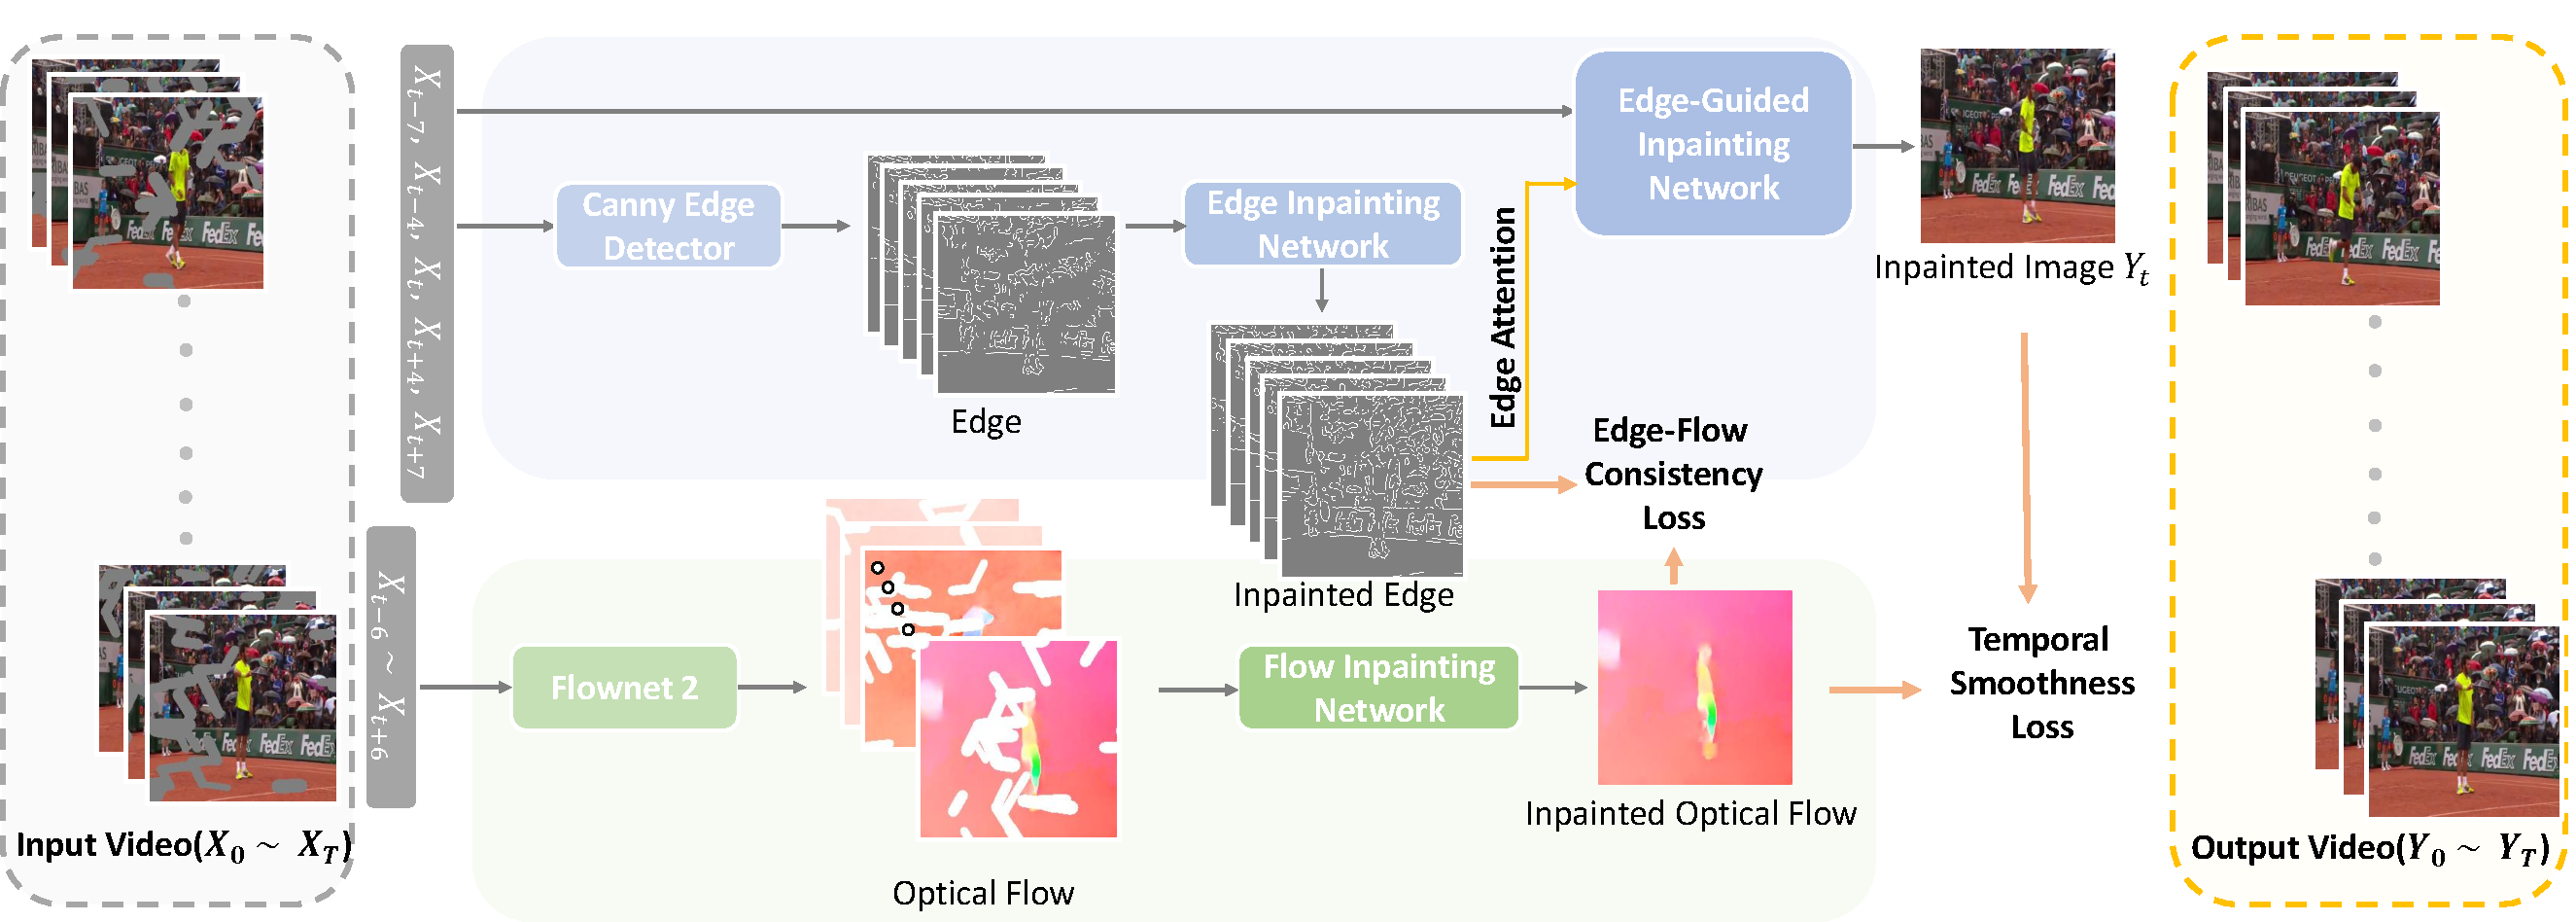
\includegraphics[width=1.0\columnwidth]{zong} % Reduce the figure size so that it is slightly narrower than the column. Don't use precise values for figure width.This setup will avoid overfull boxes. 
	\caption{The overall pipeline of SOVI. The ENet first completes the missing edge across frames. Then, under the guidance of structural edge, TexNet can produce structure-preserved inpainting frame. Moreover, the FNet is designed to predict missing optical flow, which provides temporally consistency to the final result.}
	\label{zong}
\end{figure}


To exploit complementary information across neighboring frames, traditional patch-based methods \cite{patwardhan2007video,wexler2004space,newson2014video} recurrently copy similar patches from unmasked regions and past them to the missing regions. 
This kind of method depends on a strong hypothesis that the missing content have precisely appeared in neighboring frames, which limits their generalization.
Recently, deep-learning based methods achieve state-of-the-art performance by treating a video as a 3D volume.
They utilize 3D convolution layers to predict missing content with smooth motion \cite{wang2019video}.
Among these methods, optical flow is commonly used to temporally smooth the inpainted contents \cite{Xu_2019_CVPR,Kim_2019_CVPR,Kim_2019_CVPR1} by aggregating the contextual information from neighboring frames.
By introducing motion knowledge, the above methods give promising inpainting results with temporal consistence.
However, structural  rationality is also a significant factor for realistic video inpainting. Existing methods implicitly learn to reconstruct structure during texture generation, which tend to generate over-smoothed regions. 
Similar observations are obtained in image inpainting \cite{Xiong_2019_CVPR,nazeri2019edgeconnect}. %\cite{iizuka2017globally,liu2018partialinpainting,yu2018free}. 
To solve this problem, they propose to predict object contours or edges as auxiliary information.
Despite structure-preserved image inpainting, it remains an open problem of how to simultaneously explore the structure and motion information in videos.
%However, when it comes to videos, 
%it is non-trivial to manage correlation between edge, motion and texture inpainting.
%applying image inpainting methods in a frame-by-frame manner will cause serious flickering artifacts. Besides, the problem of how to utilize structure information in video inpainting effectively is also non trivial.
%just  learned with texture and flow generation by existing methods.
%Thus, how to obtain fine-detailed inpainting video remains an open problem.
%is hard to capture the detailed information accurately. 

%has been proven to generate over-smoothed regions in \cite{nazeri2019edgeconnect}
%Besides, complementary information brought by optical flow also lacks structure guidance when the contents are missed in neighboring frames.








In this paper, we present a novel structure-oriented video inpainting network (SOVI) that can collect and exploit the structure information to improve video inpainting results. %SOVI extracts fine-detailed structure and the information
The key insight of SOVI is to explore the correlation among structure, motion, and texture for simultaneously fine-detailed and temporal coherent video generation. %This is significant departure from existing works [], where the texture is only associated with motion or structure.
%We  predict the edges, which well represents structure information. To embed  
%\cxj{Explain more about the concept. not the modules.}
As shown in Fig.~\ref{zong}, our method consists of three modules, which are respectively the edge inpainting network (ENet), flow inpainting network (FNet), and texture inpainting network (TINet).
Given frames with missing pixels, ENet first completes the edge maps that indicate the detailed structure information. Then, under the guidance of completed edge, TexNet is developed to fill the missing colors and textures in a coarse-to-fine manner.
Specifically, a structure attention module is designed to capture the latent spatial relevance between video textures and structure edges.
Compared with original edge maps, the structure-texture relevance is easier to be embedded into TexNet, which benefits fine-detailed frame generation.
Besides, the developed FNet can predict the missing optical flow, which provides auxiliary motion knowledge. Explicitly, a flow-edge consistency constraint and a temporal ensemble module are utilized to smoothen the edge maps and final inpainted frames, based on the motion tendency. Consequently, the inpainted frames by SOVI are not only detail-preserved but also temporal consistent.
%\cxj{This is about 'how', not about 'why'.}
%by simultaneously exploring optical flow and , to eliminate temporal flickers and enhance spatial detail. 
%  and FNet  and optical flow,  knowledge and motion tendency.
%according to learned structure knowledge and motion tendency from the training data,
%Instead of separate training, these two modules are
%This results in both edge-enhanced optical flow and temporally smooth edge. 
%Specifically, a structure enhancement mechanism is developed to extract and refine the structural clues in the completed edge and encode them into the STI.
% the optical flow is used by propagating complementary pixels from neighboring frames to current frame to alleviate artificial flickers and jitters.


%In summary, we present a novel structure-oriented video inpainting method, which can generate structural reasonable and temporal coherent inpainted frames.
%
Experiments on YouTubeVOS and DAVIS datasets show that the proposed method obtains new state-of-the-art performance with low time consumption, which demonstrates its superiority.
%
Our contributions can be summarized as follows:
\begin{itemize}
	\item We propose a novel structure-oriented video inpainting method, which combines edge completion, motion generation, and video inpainting for simultaneous fine-details and temporal consistency.
	\item A novel structure attention module is designed to capture the spatial relevance between video contents and structure edges, which is easily to be embedded into video inpainting network. %With edge collection and structure embedding, we demonstrate the significance of detailed structure in video inpainting. 
	%to structure information is well represented and encoded in video inpainting via . 
	\item A flow-guided warping and temporal ensemble module are developed to enhance temporal consistency for video inpainting.%, with a flow inpainting network.
	%	Optical flow is used to enhance temporal consistency, which 
	
	
	%	We propose a novel structure- for video inpainting, by simultaneously exploring optical flow and structural clues to eliminate temporal flickers and enhance structure detail. 
	%	 A flow-edge consistency loss is developed to associate the optical flow and structure edges, which can boost each other.
	%	\item  a structure enhancement mechanism is  designed, which can promote the video inpainting.	
	
\end{itemize}





\section{Related Work}
\subsubsection{Traditional Image/Video Inpainting.}
Traditional image and video inpainting methods can be divided into two categories, diffusion-based and patch-based methods. 
Diffusion-based methods \cite{bertalmio2000image,ballester2001filling} gradually propagate contents from surrounding areas to the missing regions. 
However, this kind of method fails to handle large holes due to error accumulation. 
Patch-based methods~\cite{bertalmio2003simultaneous,efros2001image} formulate the completion task as a patch-based optimization problem, which is more widely used. 
It fills the missing image contents by borrowing and aggregating the most similar patches from known regions. 
\cite{patwardhan2007video} further extends the task to video inpainting by searching patches in across frames. \cite{newson2014video} enhances the quality of video inpainting by using a video version of PatchMatch algorithm \cite{barnes2009patchmatch}. 
Then, \cite{huang2016temporally} proposes completing the missing optical flow to alleviate the temporal artifacts and enforce temporal consistency. 
However, traditional methods assume that there should exist complementary contents in known regions, which can not synthesize unseen appearances. Besides, the propagation process makes these methods suffer from high computational complexity, which limits their usage in practical applications. 

\subsubsection{CNN-based Image/Video Inpainting.}
Recently, deep learning methods  have achieved tremendous progress because of their capability of capturing high-level semantic information of images and videos. 
first introduces 
The convolution neural network (CNN) is first introduced to synthesize small unknown regions and denoise in images \cite{xie2012image}. 
To improve the photorealism of the completed results, a generative adversarial network is employed \cite{pathak2016context} by jointly training a generator and a discriminator in a minimax manner. 
Then, \cite{iizuka2017globally} proposes using two discriminators to constrain both global and local coherence of image contents. Later, \cite{liu2018partialinpainting} designs partial convolution to handle holes of irregular shapes. \cite{yu2018free} introduces gated convolution to learn a dynamic feature selection mechanism in CNN.
%However, methods aforementioned usually handle the square masks, which produce artificial when recovering challenging holes of irregular shapes. 
%\cxj{What is the underlying difference between these two mask shapes?}
%
%%% irregular  masks
%To solve this,
%. Later, \cite{yu2018free} introduces gated convolution to learn a dynamic feature selection mechanism in CNN.  
\cite{nazeri2019edgeconnect} introduces an edge generator to refine generated structure in image inpainting. These image inpainting methods can obtain plausible synthesized images. 
%\cxj{In comparison, what is the difference of our method when sovling irregular masks?}


%%% video inpainting 
However, directly extending these state-of-the-art image inpainting methods to video domain is not an optimal solution, which will generate videos with serious temporal flickers, artifacts and jitters. Besides, Image inpainting methods can not utilize useful complementary information in neighboring frames. To obtain spatio-temporal consistent inpainted video, some methods have been proposed recently.
\cite{wang2019video} proposes CombCN to capture both temporal and spatial consistency, which is the first to use CNN-based method in video inpainting. \cite{Xu_2019_CVPR} proposes a stacked convolution network to predict missing motion field and regards video inpainting as a pixel propagation problem. \cite{Kim_2019_CVPR} automatically removes texts in videos without mask indications, which aggregates temporal features from encoder to decoder and applies a recurrent feedback. \cite{Kim_2019_CVPR1} introduces convolutional LSTM and temporal feature aggregation to obtain temporal consistency and learn information from neighboring frames. However, these existing methods neglect the importance of structure information in video inpainting, which will cause the blurry details and structural cracks in generated videos. 

Different from the methods above, SOVI extract and refine structure information explicitly, which will generate fine-detailed video inpainting results.
%predict edge maps explicitly, which well represent structure details. 
%\cxj{What is our key difference?}


\dlt{
	To tackle these issues, we propose a novel structure-oriented video inpainting network (SOVI) based on CNN.
	Different from the methods above, SOVI
	takes the effect of structure information into consideration. In our network, we collect and refine the structure information to enhance the final generated video. Specifically, a structure attention module is introduced to learn latent correlation between video contents and structure. Besides, temporal consistency is also guaranteed through flow-guided warping and temporal ensemble module. Finally, we can generate spatio-temporal consistent inpainted video. 
}






























%\section{Introduction}
%
%
%Video inpainting aims to recover the missing contents of given videos, which can assist lots of practical applications, e.g., video restoration and augmented reality. The task requires not only reasonable spatial structures but also temporal consistency. 
%
%Existing video inpainting methods exploit structural information by propagating complementary information across neighboring frames implicitly. \cite{patwardhan2007video,wexler2004space,newson2014video} recurrently copy similar patches from unmasked regions and past them to the missing regions. This kind of method depends on a strong hypothesis that the missing contents have precisely appeared in neighboring frames, which limits their generalization. Recently, deep-learning based methods achieve state-of-the-art performance by treating a video as a 3D volume. They utilize 3D convolution layers to predict video frames \cite{wang2019video}. Among these methods, optical flow is commonly used to propagate appearances by aggregating the contextual information from neighboring frames \cite{Xu_2019_CVPR,Kim_2019_CVPR,Kim_2019_CVPR1}.
%However, the missing structural details can not be created by motion compensation. 
%Thus, the auxiliary information brought by optical flow lacks detailed structural clues, e.g. the inner textures of objects are usually missed in flow field, leading to deficient structure rationality and video blurs.
%
%Image inpainting methods \cite{Xiong_2019_CVPR,nazeri2019edgeconnect} predict object contours or edges for structure enhancement. Though these methods can obtain sharp-detailed images to some degrees, directly applying these approaches to each individual frame in video inpainting will lead to serious artifacts, flickers and jitters.  Thus, how to obtain fine-detailed inpainting video remains an open problem.
%%Compared with image inpainting, video inpainting is much more challenging due to the extra time dimension. 
%%\mdf{Though great progress has been made in 2D image inpainting using deep learning techniques \cite{yu2018free,Xiong_2019_CVPR}, directly applying these approaches to each individual frame in video inpainting could lead to artifacts, flickers and jitters. }
%
%In this paper, we present a novel structure-oriented video inpainting network (SOVI) that can collect and refine the structure information to improve the inpainting results. 
%The proposed SOVI is based a 3-node graph of motion, structure, and texture. This is based on the key insight that the structure and motion are two significant factors for a realistic video content. This is significant departure from existing works \, where the texture is only associated with motion or structure.
%
%%To exploit complementary information across neighboring frames, traditional patch-based methods \cite{patwardhan2007video,wexler2004space,newson2014video} recurrently copy similar patches from unmasked regions and past them to the missing regions. 
%%This kind of method depends on a strong hypothesis that the missing content have precisely appeared in neighboring frames, which limits their generalization.
%Recently, deep-learning based methods achieve state-of-the-art performance by treating a video as a 3D volume.
%%They utilize 3D convolution layers to predict missing content with smooth motion \cite{wang2019video}.
%%Among these methods, optical flow is commonly used to temporally smooth the inpainted contents \cite{Xu_2019_CVPR,Kim_2019_CVPR,Kim_2019_CVPR1} by aggregating the contextual information from neighboring frames.
%%However, the auxiliary motion compensation brought by optical flow lacks detailed structural clues, e.g. the inner textures of objects are usually missed in flow field, leading to deficient structure rationality.
%%\cxj{It is not clear why motion compensation lacks structural clues..}
%Thus, how to obtain fine-detailed inpainting video remains an open problem.
%
%
%
%
%\begin{figure}[t]
%	\centering
%	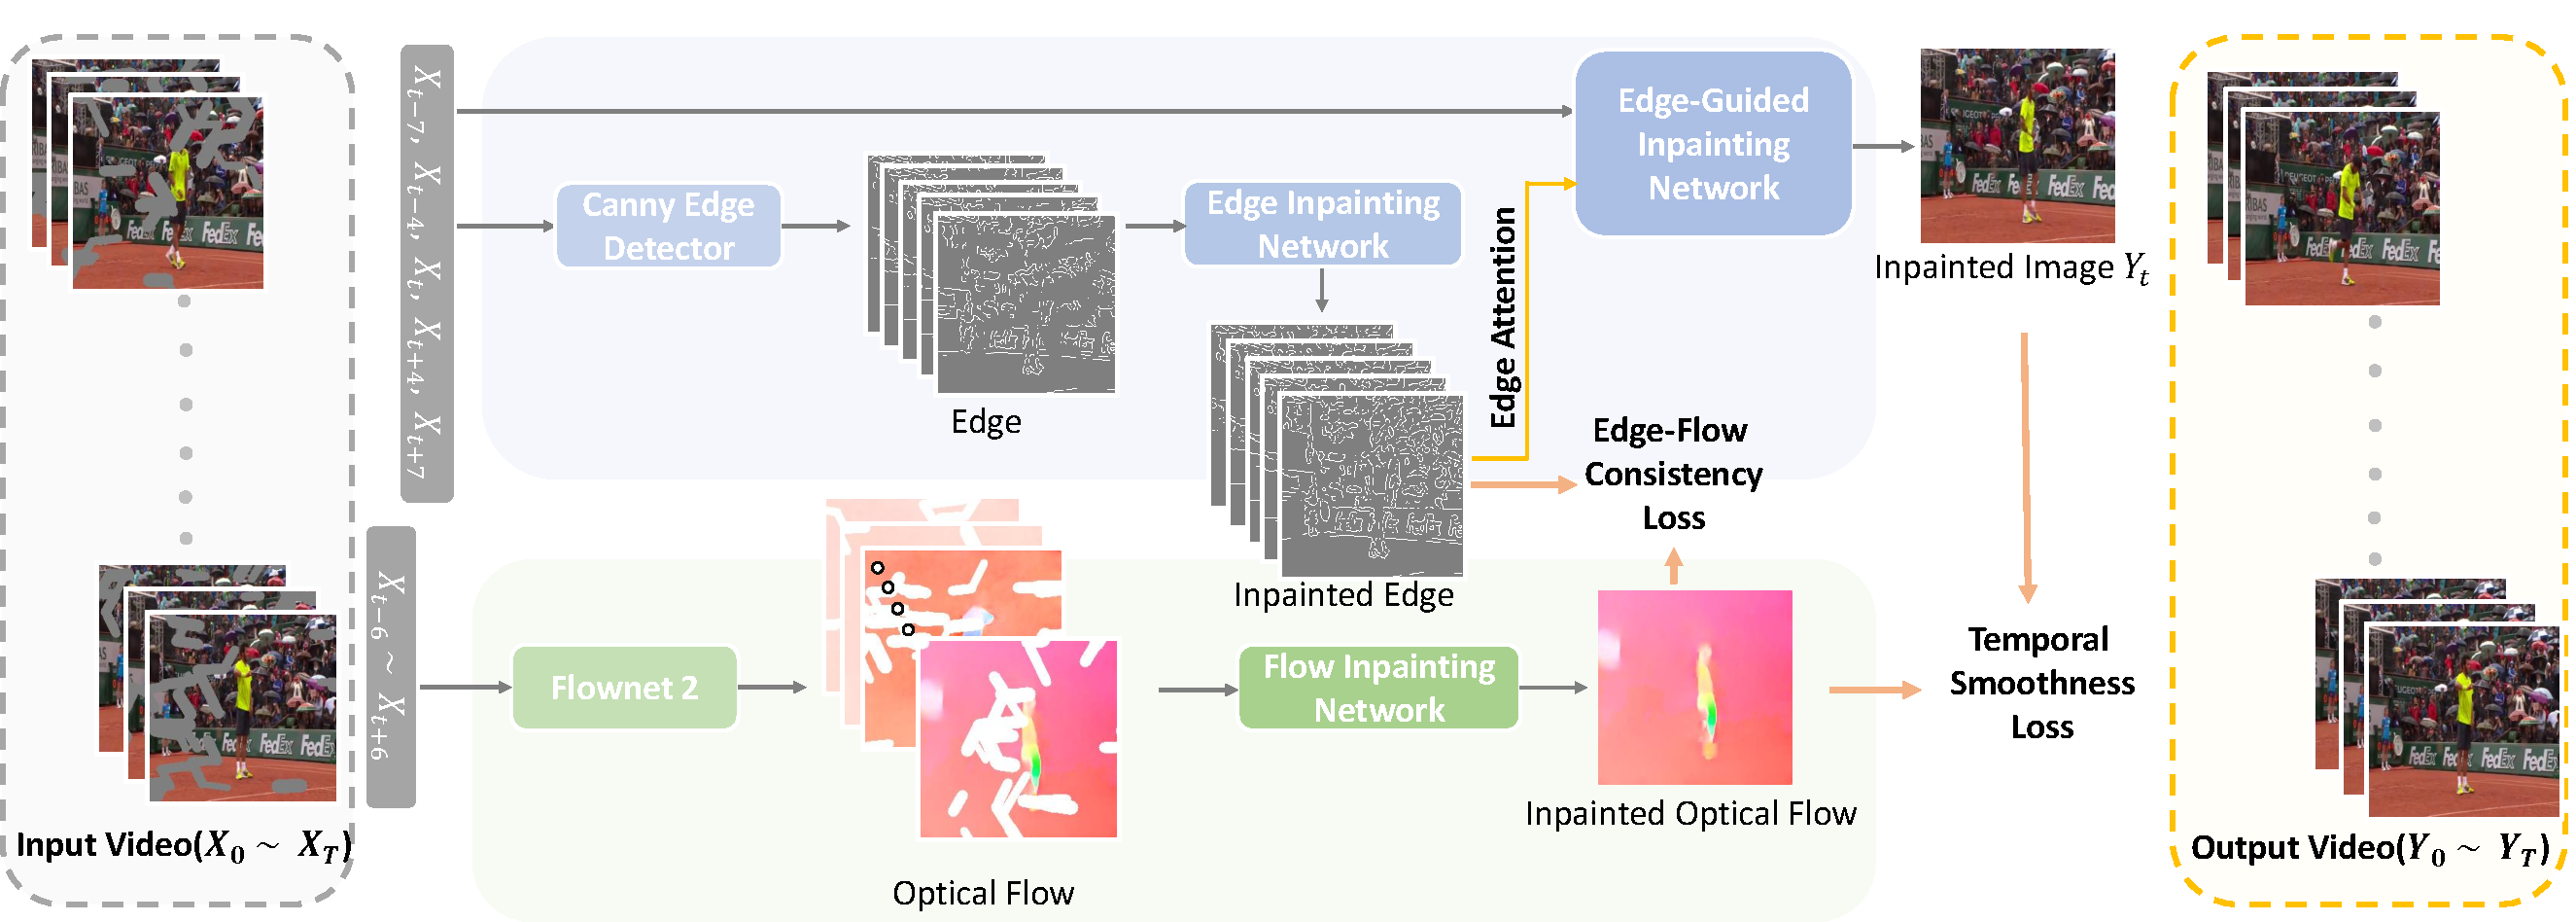
\includegraphics[width=1.0\columnwidth]{zong} % Reduce the figure size so that it is slightly narrower than the column. Don't use precise values for figure width.This setup will avoid overfull boxes. 
%	\caption{The overall pipeline of SOVI. The ENet first completes the missing edge across frames. Then, under the guidance of structural edge, TexNet can produce structure-preserved inpainting frame. Moreover, the FNet is designed to predict missing optical flow, which provides temporally consistency to the final result.}
%	\label{zong}
%\end{figure}
%
%
%In this paper, we present a novel structure-oriented video inpainting network (SOVI) that can collect and refine the structure information to improve the inpainting results. 
%\cxj{Explain more about the concept. not the modules.}
%As shown in Fig.~\ref{zong}, our method consists of three modules, which are respectively the edge inpainting network (ENet), flow inpainting network (FNet), and spatio-temporal inpainting network (TINet).
%Given frames with missing pixels, ENet first completes the edge maps that indicate the detailed structure information. Then, under the guidance of completed edge, TexNet is developed to fill the missing colors and textures in a coarse-to-fine manner.
%Specifically, a structure attention module is designed to capture the latent spatial relevance between video contents and structure edges.
%Compared with original edge maps, the structure-texture relevance is easier to be embedded into TexNet, which benefits fine-detailed frames generation.
%Besides, the developed FNet can predict the missing optical flow, which provides auxiliary motion knowledge. Explicitly, a flow-edge consistency constraint and a temporal ensemble module are utilized to smoothen the edge maps and final inpainted frames, based on the motion tendency. Consequently, the inpainted frames by SOVI are not only detail-preserved but also temporal consistent.
%\cxj{This is about 'how', not about 'why'.}
%%by simultaneously exploring optical flow and , to eliminate temporal flickers and enhance spatial detail. 
%%  and FNet  and optical flow,  knowledge and motion tendency.
%%according to learned structure knowledge and motion tendency from the training data,
%%Instead of separate training, these two modules are
%%This results in both edge-enhanced optical flow and temporally smooth edge. 
%%Specifically, a structure enhancement mechanism is developed to extract and refine the structural clues in the completed edge and encode them into the STI.
%% the optical flow is used by propagating complementary pixels from neighboring frames to current frame to alleviate artificial flickers and jitters.
%
%
%In summary, we present a novel structure-oriented video inpainting method, which can generate structural reasonable and temporal coherent inpainted frames.
%%
%Experiments on YouTubeVOS and DAVIS datasets show that the proposed method obtains new state-of-the-art performance with low time consumption, which demonstrates its superiority.
%%
%This improvement derives from two technical contributions:
%\begin{itemize}
%
%\item We introduce an edge inpainting network to predict the missing edges. Besides, a novel structure attention module is designed to capture the spatial relevance between video contents and structure edges, which is easily to be embedded into video inpainting network. %With edge collection and structure embedding, we demonstrate the significance of detailed structure in video inpainting. 
%	%to structure information is well represented and encoded in video inpainting via . 
%\item A flow-guided warping and temporal ensemble module are developed to enhance temporal consistency for video inpainting, with a flow inpainting network.
%	%	Optical flow is used to enhance temporal consistency, which 
%
%	
%	%	We propose a novel structure- for video inpainting, by simultaneously exploring optical flow and structural clues to eliminate temporal flickers and enhance structure detail. 
%	%	 A flow-edge consistency loss is developed to associate the optical flow and structure edges, which can boost each other.
%	%	\item  a structure enhancement mechanism is  designed, which can promote the video inpainting.	
%	
%\end{itemize}
%
%
%
%
%
%\section{Related Work}
%\subsubsection{Traditional Image/Video Inpainting.}
%Traditional image and video inpainting methods can be divided into two categories, diffusion-based and patch-based methods. 
%Diffusion-based methods \cite{bertalmio2000image,ballester2001filling} gradually propagate contents from surrounding areas to the missing regions. 
%However, this kind of method fails to handle large holes due to error accumulation. 
%Patch-based methods~\cite{bertalmio2003simultaneous,efros2001image} formulate the completion task as a patch-based optimization problem, which is more widely used. 
%It fills the missing image contents by borrowing and aggregating the most similar patches from known regions. 
%\cite{patwardhan2007video} further extends the task to video inpainting by searching patches in across frames. \cite{newson2014video} enhances the quality of video inpainting by using a video version of PatchMatch algorithm \cite{barnes2009patchmatch}. 
%Then, \cite{huang2016temporally} proposes completing the missing optical flow to alleviate the temporal artifacts and enforce temporal consistency. 
%However, traditional methods assume that there should exist complementary contents in known regions, which can not synthesize unseen appearances. Besides, the propagation process makes these methods suffer from high computational complexity, which limits their usage in practical applications. 
%
%\subsubsection{CNN-based Image/Video Inpainting.}
%Recently, deep learning methods  have achieved tremendous progress because of their capability of capturing high-level semantic information of images and videos. 
%% first introduces 
%The convolution neural network (CNN) is first introduced to synthesize small unknown regions and denoise in images \cite{xie2012image}. 
%To improve the photorealism of the completed results, a generative adversarial network is employed \cite{pathak2016context} by jointly training a generator and a discriminator in a minimax manner. 
%Then, \cite{iizuka2017globally} proposes using two discriminators to constrain both global and local coherence of image contents. 
%However, methods aforementioned usually handle the square masks, which produce artificial when recovering challenging holes of irregular shapes.
%\cxj{What is the underlying difference between these two mask shapes?}
%%
%
%%%% irregular  masks
%To solve this,
% \cite{liu2018partialinpainting} designs a network which utilizes the partial convolution. Later, \cite{yu2018free} introduces gated convolution to learn a dynamic feature selection mechanism in CNN.  \cite{nazeri2019edgeconnect} introduces an edge generator to refine generated structure in image inpainting. These image inpainting methods can obtain plausible synthesized images. 
%\cxj{In comparison, what is the difference of our method when sovling irregular masks?}
% 
%
%%%% video inpainting 
% However, directly extending these state-of-the-art image inpainting methods to video domain is not an optimal solution, which will generate videos with serious temporal flickers, artifacts and jitters. Besides, image inpainting methods can not utilize useful complementary information in neighboring frames. To obtain spatio-temporal consistent inpainted video, some methods have been proposed recently.
%\cite{wang2019video} proposes CombCN to capture both temporal and spatial consistency, which is the first to use CNN-based method in video inpainting. \cite{Xu_2019_CVPR} proposes a stacked convolution network to predict missing motion field and regards video inpainting as a pixel propagation problem. \cite{Kim_2019_CVPR} automatically removes texts in videos without mask indications, which aggregates temporal features from encoder to decoder and applies a recurrent feedback. \cite{Kim_2019_CVPR1} introduces convolutional LSTM and temporal feature aggregation to obtain temporal consistency and learn information from neighboring frames. However, these existing methods neglect the importance of structure information in video inpainting, which will cause the blurry details and structural cracks in generated videos. 
%\cxj{What is our key difference?}
%
%
%
%\dlt{
%To tackle these issues, we propose a novel structure-oriented video inpainting network (SOVI) based on CNN.
% Different from the methods above, SOVI
%takes the effect of structure information into consideration. In our network, we collect and refine the structure information to enhance the final generated video. Specifically, a structure attention module is introduced to learn latent correlation between video contents and structure. Besides, temporal consistency is also guaranteed through flow-guided warping and temporal ensemble module. Finally, we can generate spatio-temporal consistent inpainted video. 
%}






\section{Approach}
\label{sec:approach}

The target of our method is to recover the missing contents in a corrupted video with fine details and temporal consistence.
%
%Our intuition is that there exists complementary information in neighboring frames, which can benefit the inpainting process of each individual frame.Therefore, 
In each inference batch to fill up the missing part in frame $X_t$, total $T$ frames $\boldsymbol{X}$ ($T=5$), indexed by $\msset{X}$, are fed to our inpainting network, as well as the corresponding masks $\boldsymbol{M}$ that indicate the missing regions.
The final output is the completed frame \(Y_t\) at time $t$. 
%Our method infers each target frame $Y_t$ individually but with hints from its neighboring source frames.
%To fill up the missing region with structural details and temporal coherence, 
As Fig.~\ref{fig:stiNet} shows, our network consists of two paths. 
The first is an edge-guided inpainting path, which consists of an edge inpainting network ENet that recovers missing edges of the input frames, a coarse-to-fine texture inpainting network TexNet that replenishes appearance details under the structure guidance.
The second path leverages motion flows to enhance temporal coherence of the completed frames.
It consists of a flow inpainting network FNet that predicts the motion flows in the missing regions and an ensemble module that aggregates previously synthesized frames to refine the current frame. 



\subsection{Edge Inpainting Network}
\label{sec:edgenet}
 
To fill the missing regions with fine details, their corresponding structural edges are predicted, and provide structural guidance for the following texture synthesis.
%
Given the input corrupted frames $\boldsymbol{X}$, a canny edge detector is first used to extract the edge maps $\boldsymbol{E}^{i}$. %Notably, the edges in the masked regions in $\boldsymbol{E}^{i}$ are missed. 
%Given the incompleted grayscale images $\boldsymbol{X}^{g}$ of input frame, a canny edge detector is first used to generate initial edge maps . 
Then, the ENet completes the missing edges.
The input of ENet consists of the grayscale frames $\boldsymbol{X}^{g}$, initial edge maps $\boldsymbol{E}^{i}$, and their corresponding masks $\boldsymbol{M}$.
%
As shown in Fig.~\ref{fig:stiNet}, ENet consists of a generator $G^E$ and a discriminator $D^E$.
$G^E$ is composed of a two-layer 3D encoder, eight 2D residual blocks, and a two-layer 3D decoder. 
The 3D encoder and decoder are designed to learn the spatio-temporal correlation, while the 2D residual blocks are used to enrich spatial features in larger receptive fields. The discriminator $D^E$ follows the $70\times 70$ PatchGAN architecture \cite{Isola_2017_CVPR}. 
Finally, the inpainted edge maps are obtained by:
\begin{equation}
\label{eq:edgenet}
\boldsymbol{E}=G^E(\boldsymbol{E}^{i},\boldsymbol{X}^{g},\boldsymbol{M}).
\end{equation}

The ENet is trained by playing a minimax game to optimize the generator $G^E$ and the discriminator $D^E$ as
\begin{equation}
\label{eq:loss_e}
\mathcal{O}_{edge} =\min\limits_{G^E} \max \limits_{D^E} \big(\mathcal{L}^E_{adv}+\lambda_1 * \mathcal{L}^E_{fm}\big),
\end{equation}
where $\mathcal{L}^E_{adv}$ and $\mathcal{L}^E_{fm}$ are the adversarial loss and feature matching loss. 
$\lambda_1$ is a hyper-parameter to balance the three terms.
%
Following the adversarial learning manner, $\mathcal{L}^E_{adv}$ can facilitate ENet to produce plausible edge maps by:
\begin{equation} \label{eq:edge_adver}
\begin{aligned} 
\mathcal{L}^E_{adv}  =&\mathbb{E}_{(\boldsymbol{E}^{gt},\boldsymbol{X}^{g})}\big[logD^E(\boldsymbol{E}^{gt},\boldsymbol{X}^{g})\big]\\ 
+&\mathbb{E}_{(\boldsymbol{E},\boldsymbol{X}^{g})}\big[log\big(1-D^E ( \boldsymbol{E},\boldsymbol{X}^{g})\big)\big],
\end{aligned}
\end{equation}
where $\boldsymbol{E}^{gt}$ represents the ground truth edge maps. $\mathcal{L}^E_{fm}$ evaluates the feature-level similarity between ground truth edge maps and predicted edge maps, which helps to create structurally rational edge maps. 
Feature matching loss was first proposed in \cite{wang2018high} and has been widely used in recent GANs.
The feature matching loss is defined as:
\begin{equation}
\label{eq:edge_fm}
\mathcal{L}^E_{fm}=\sum_{k=1}^L{\frac{1}{N_k}\left\| D^E_k(\boldsymbol{E}^{gt},\boldsymbol{X}^{g})- D^E_k(\boldsymbol{E},\boldsymbol{X}^{g})\right\|_1},
\end{equation}
where $D^E_k$ is the output of the $k$-th layer in $D^E$, while $N_k$ is the element number of $D^E_k$. 
%Note that the discriminator $D^E$ is not optimized by the feature matching loss term. It plays as a feature extractor to optimize the generator $G^E$ for producing plausible edge maps $\boldsymbol{E}$.


\begin{figure}[t]
	\centering
	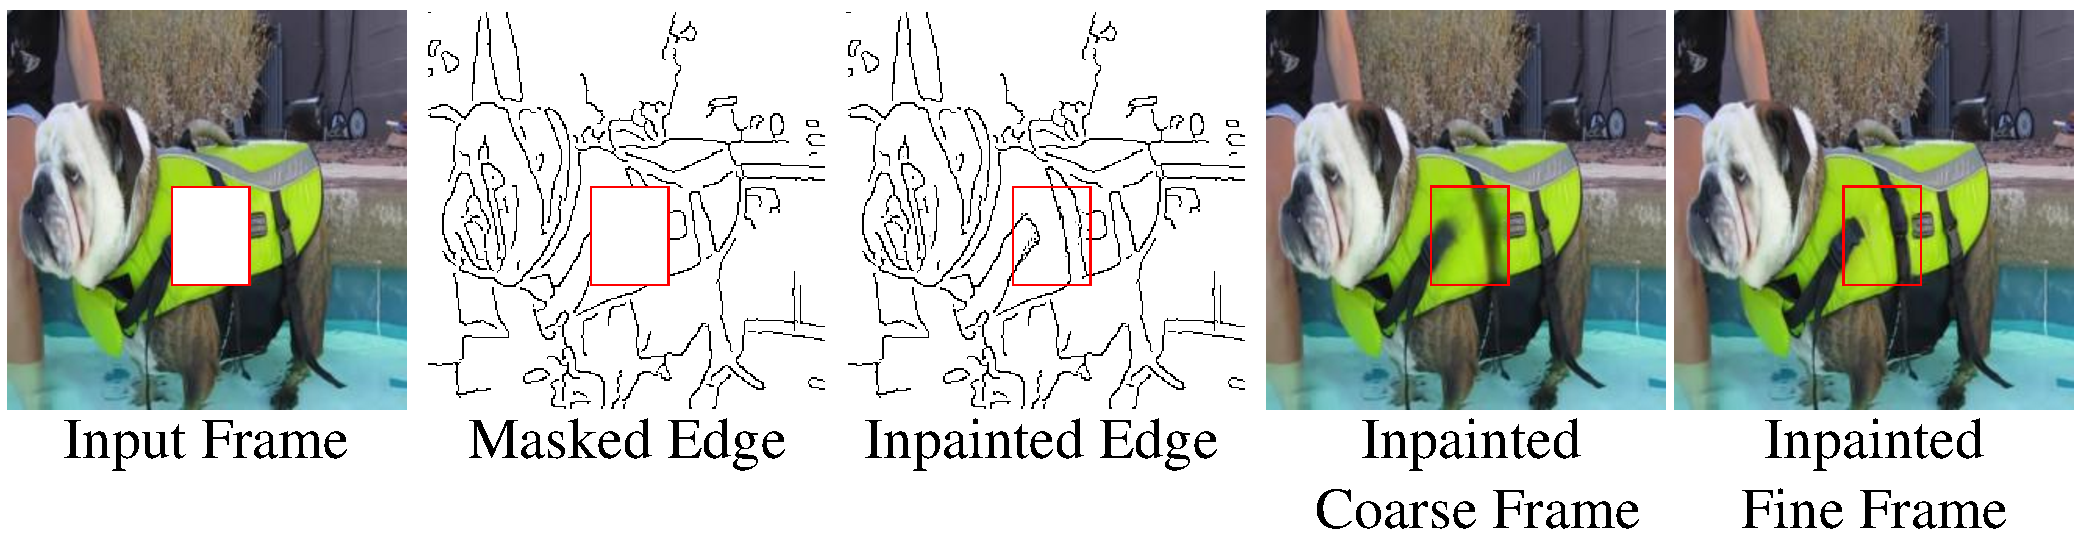
\includegraphics[width=1.0\columnwidth]{coars-fine} % Reduce the figure size so that it is slightly narrower than the column. Don't use precise values for figure width.This setup will avoid overfull boxes. 
	\caption{Given a corrupted frame (a), our ENet first completes sparse edges (b) which well represent the structure of the missing content. Then TexNet progressively replenishes textures under the guidance of synthesized edges from coarse (c) to fine (d).}
	
	\label{fig:coarse-fine}
\end{figure}



\subsection{Edge-Guided Texture Inpainting Network}

%Combining the inpainted edge maps $\boldsymbol{E}$ and flow maps $\boldsymbol{O}$, a spatio-temporal inpainting network (STINet) is designed to obtain the final target frame $Y_t$.

Given the completed edge maps $\boldsymbol{E}$ for the 
$T$ frames, then we fill textures under the structural guidance in a coarse-to-fine manner. 
%
The proposed TexNet consists of a coarse network and a refinement network, as Fig.~\ref{fig:stiNet} shows.
%
The input of TexNet is the concatenation of $\boldsymbol{X}$, $\boldsymbol{E}$, and $\boldsymbol{M}$.
First, the coarse inpainting network consists of a set of 3D convolutions to capture the temporal information, which targets to produce an rough completion for the $T$ frames  $\boldsymbol{Y}^i$ with colors.
%The 3D coarse network incorporates neighboring frames by convolutions of the time dimension.
Second, the refinement network takes the synthesized edge maps $\boldsymbol{E}$, $\boldsymbol{Y}^i$ and $\boldsymbol{M}$ as input and uses 2D convolutions to enhance structure details and synthesize frame $Y^T_t$. 
%For the corrupted region, our ENet first completes sparse edges which well represent the structure of the missing content, then TexNet progressively replenishes textures under the guidance of synthesized edges.



To fully exploit the structural information in $\boldsymbol{E}$, we design a structure attention module (SAM) in the refinement network.
The core insight of the SAM is to capture the spatial correlation between edges and textures.
The detailed implementation of the SAM is given in Fig.~\ref{SEM}.
%Two separate convolution blocks are first applied to embed structure features from the predicted edge maps $\boldsymbol{E}$.
% which alleviate the feature discrepancy between structural edge and video texture.
The intermediate video features and embedded edge features are interacted to calculate the latent structure-texture correlation via matrix multiplication. 
%After a SoftMax operation, the normalized attention map represents long-range correlation between the structure and high-level video features.
%
The normalized attention map is applied to the intermediate video features, and the structure information is thus embedded in TexNet.
After introducing structural guidance, the inpainted content by TexNet becomes more structurally and semantically realistic, as Fig.~\ref{fig:coarse-fine} shows.
%Fig.~\ref{fig:coarse-fine} shows an example of our structure-guided inpainting result. 
 


To train the TexNet, we define the loss function as:
%
\begin{equation}
	\label{eq:1}
		\mathcal{O}_{tex}=\min\limits_{G^T} \max \limits_{D^T} \big(\mathcal{L}^{T}_{rec}+\mathcal{L}^T_{adv}\big).
\end{equation}
%
Inspired by \cite{nazeri2019edgeconnect}, the first term $\mathcal{L}^{T}_{rec}$ is the $l_1$-reconstruction loss to measure the difference between predicted video frames and the ground truth video frames $\widetilde{\boldsymbol{Y}}$.
Different from \cite{nazeri2019edgeconnect}, we penalize both the coarse predictions $\boldsymbol{Y}^i$ and refined frame $Y^{T}_t$, given by:
\begin{equation}
	\begin{aligned}
		\mathcal{L}^{T}_{rec}&=\frac{1}{\left\|\boldsymbol{M} \right\|_1}\left\|(\boldsymbol{Y}^i-\widetilde{\boldsymbol{Y}})\odot \boldsymbol{M}\right\|_1\\ &+\lambda_2*\frac{1}{\left\|M_t \right\|_1}\left\|(Y^T_t-\widetilde{Y}_t)\odot M_t\right\|_1.
	\end{aligned}
\end{equation}
%
%
Besides, an extra adversarial loss $\mathcal{L}^T_{adv}$ is introduced to promote the visual realism of the generated frame.
\dlt{ by:
%$\mathcal{L}^I_{adv}$ is defined as:
\begin{equation}
	\label{eq:inp_adver}
	\mathcal{L}^I_{adv}=\mathbb{E}[logD^I(\widetilde{Y}_t)]+\mathbb{E}[log\big(1-D^I(Y^I_{t})\big)],
\end{equation}
where $G^I$ is the TexNet and $D^I$ has the similar architecture with $D^E$.}
% $\mathcal{L}^I_{adv}$ enforces the generated frame to be more realistic.





 \begin{figure}[t]
	\centering
	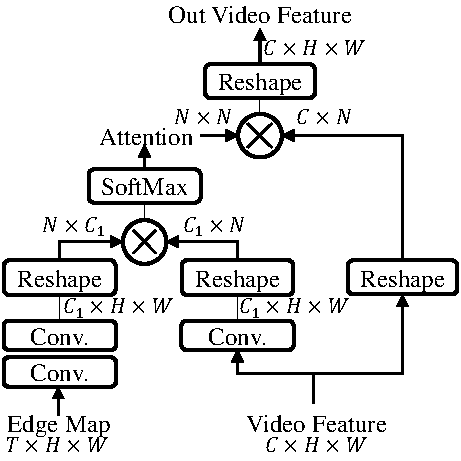
\includegraphics[width=0.7\columnwidth]{SEM} % Reduce the figure size so that it is slightly narrower than the column. Don't use precise values for figure width.This setup will avoid overfull boxes. 
	\caption{Architecture of the structure attention module. $C$ is the channel of the input video features, and $N=H\times W$. $\otimes$ represents matrix multiplication. Usually, we set $C_1=C/8$.}
	\label{SEM}
\end{figure} 


\begin{table*}[t]
	\caption{Comparisons with existing methods on YouTubeVOS. To save space, the year of method is not listed.}\smallskip
	
	\centering
	\resizebox{2.0\columnwidth}{!}{
		\smallskip\begin{tabular}{c|c|c|c|c|c|c|c|c|c|c }
			\hline
			&\multicolumn{3}{c|}{Fixed Square Mask}& \multicolumn{3}{c|}{Moving Square Mask}&\multicolumn{3}{c|}{Free-Form Mask}&Inference \\
			\cline{2-10} 
			&PSNR & SSIM & FID & PSNR & SSIM & FID & PSNR & SSIM & FID&Speed(fps))\\
			\hline
			Nazeri et al. &28.6446 &0.9484  &   38.2116  &	
			30.7478 & 0.9647 &  16.2739  &
			25.6693  & 0.9088 &  43.0366&22.81 \\
			\hline
			Wang et al. &27.9668 & 0.9515 &  40.7199  &	 
			31.5776	& 0.9678 &  13.8383&   
			32.1862 & 0.9626 & 19.1191 &8.1634 \\
			\hline
			
			
			Kim et al. b& 28.0846&0.9468 &  39.9377  & 
			36.8598	& 0.9728 &7.2315  &
			33.5549	& 0.9646 & 9.3797&1.2275  \\
			\hline
			Xu et al. &29.0531 & 0.9497 &  32.8860  & 
			37.8241& 0.9772 &6.3746  &
			32.6287 &0.9618  &  11.1501&0.5620 \\
			\hline
			
			\hline
			
			
			TexNet &28.0174 &0.9494  &  42.7164   &	
			33.8131 &  0.9705  &8.2390	& 
			30.0680& 0.9390 & 20.6358&7.6335
			\\
			\hline
			+edge input  &29.5242 &  0.9520& 36.2097   &	
			37.6630	& 0.9798 &3.5161    &	
			33.8206	&0.9659  &    6.6651& 5.2356 \\
			\hline
			
			+SAM &29.9918 &  0.9533 &  27.4198  &	
			38.2433	& 0.9807 &   2.5083  &	
			35.7783	&0.9712  &   5.8786 & 5.1546\\
			\hline
			
			
			
			
			Ours &\textbf{30.0590} &\textbf{0.9543}&   \textbf{27.2431} &
			\textbf{38.8186} & \textbf{0.9824} & \textbf{2.3455} &
			\textbf{35.9613}  & \textbf{0.9721}&  \textbf{ 5.8694} &2.5643\\
			
			\hline
			
			
		\end{tabular}
	}
	\label{tab:sem}
\end{table*}







\subsection{Flow-Guided Temporal Coherence Enhancement}
\label{sec:fec}
It is vital to maintain temporal consistency in video inpainting.
%Optical flows are widely used to represent the dense correspondence between frames.
To enhance temporal consistency in the synthesized results, we employ optical flows to smooth the inpainted edge maps and synthesized frames from ENet and TexNet.
% and reinforce the temporal coherence between neighboring edge maps and frames during training. 
Moreover, we design an ensemble module which leverages the previous inpainted frames to refine the current frame completion, as Fig.~\ref{fig:stiNet} shows. 
%
We design a flow inpainting network (FNet) to predict the optical flow in the missing region.
%
Similar to ENet, a set of initial flow maps \(\boldsymbol{O}^i\) for pairs between the current frame $X_t$ and its neighboring frames are first generated using a flow extraction network, such as FlowNet2.0~\cite{Flownet_2017_CVPR}.
Notably, \(\boldsymbol{O}^i\) consists of four flow maps \((O^i_{t\Rightarrow t-7}, O^i_{t\Rightarrow t-3}, O^i_{t\Rightarrow t+3}, O^i_{t\Rightarrow t+7})\).
From the predicted optical flows $\boldsymbol{O}^i$, FNet estimates the flows in the missing regions to obtain four flow maps \(\boldsymbol{O}\) as:
\begin{equation}
	\label{eq:flownet}
	\boldsymbol{O}=G^F(\boldsymbol{O}^{i},\boldsymbol{M}),
\end{equation}
where $G^F$ denotes FNet, which consists of an encoder that uses ResNet101 \cite{He_2016_CVPR} as backbone and a decoder.
%The detailed architecture of FNet is shown in Fig.~\ref{fig:stiNet}.

To train the flow inpainting network, the loss function is given by:
\begin{equation}
	\label{eq:flow_all}
	\mathcal{O}_{flow}=\min\limits_{G^F} \big(\mathcal{L}^F_{rec}+ \mathcal{L}^F_{har}+\mathcal{L}_{fec}\big),
\end{equation}
where $\mathcal{L}^F_{rec}$ and $\mathcal{L}^F_{har}$ are respectively $l_1$ loss and hard example mining loss in the missing regions, following the definition in \cite{Xu_2019_CVPR}. 
%Specifically, $\mathcal{L}^F_{har}$ encourages the network to focus on those hard samples in order to avoid blurry texture.




To enhance temporal consistency in the synthesized results, we apply the completed flows to warp the inpainted edge maps and compute the consistency between neighboring edge maps. 
%
Instead of separately training two subnetworks ENet and FNet, we train them jointly, because the temporal correlation and structural details can boost each other. 
To achieve this goal, a flow-edge consistency loss is defined as:
%
\begin{equation}
	\label{eq:flow_edge}
	\mathcal{L}_{fec}=\sum_{k}\frac{1}{\left\|M_{t} \right\|_1}\left\|(E_{t}-\phi(O_{t\Rightarrow t-k},E_{t-k}))\odot M_{t}\right\|_1,
\end{equation}
where $\phi(O_{t\Rightarrow t-k},E_{t-k})$ is the warping operation which warps the edge map $E_{t-k}$ to the target frame according to the generated optical flow $O_{t\Rightarrow t-k}$.
$k$ denotes the index of neighboring frames ($k\in \left\{-7,-3,+3,+7 \right\}$). Also, $\mathcal{L}_{fec}$ is added to Eq.~\eqref{eq:loss_e} for joint training of ENet and FNet.
%Specifically, $\mathcal{L}_{fec}$ warps the edge maps from neighboring frames to the target frame to penalize the reconstruction loss.
%In terms of ENet, $\mathcal{L}_{fec}$ encourages the predicted edge maps to be temporally smoothing, which should conform to the motion tendency in the flow maps $\boldsymbol{O}$. 
%In terms of FNet, $\mathcal{L}_{fec}$ constrains the model to focus on edges.
%Thus, the total loss function for joint training of ENet and FNet is:
%\begin{equation}
%	\label{eq:flow}
%	\mathcal{L}_{joint}=\mathcal{L}_{edge}+\mathcal{L}_{flow}+ \mathcal{L}_{fec}.
%\end{equation}


To eliminate temporal flickers in the completed video frames, we enforce the temporal coherence of synthesized neighboring frames via a flow warping constraint $\mathcal{L}^T_{flo}$. 
%
Specifically, the neighboring frames are warped into the target frame to compute the difference: 
\begin{equation}
\label{eq:inp_flow}
\mathcal{L}^T_{flo}=\sum_{\widehat{t}\in\mathcal{T}}\left\| Y^T_t-\phi(O_{t\Rightarrow \widehat{t}},Y_{\widehat{t}}) \right\|_1,
\end{equation}
where $\mathcal{T}=\{t-7,t-3\}$. $\phi(O_{t\Rightarrow \widehat{t}},Y_{\widehat{t}})$ warps $Y_{\widehat{t}}$ to $Y^T_{t}$ using flow $O_{t\Rightarrow \widehat{t}}$.
%$O_{t\Rightarrow \widehat{t}}$ is predicted using the subsequent flow inpainting network.
%$\mathcal{L}^I_{flo}$ expects that all the neighboring frames can be well warped to the target frame with small reconstruction loss.
%
$\mathcal{L}^T_{flo}$ is added to Eq.~\eqref{eq:1}.
Finally, a temporal ensemble module is designed 
to refine the current frame $Y_t$ by aggregating previous frames. %The architecture is shown in Fig.~\ref{fig:stiNet}. 
This module is trained with a $l_1$-reconstruction loss and an adversarial loss.










\section{Experiments}
We test on two datasets, YoutubeVOS \cite{xu2018youtube} and DAVIS \cite{davis_2017}, to compare the proposed STINet with state-of-the-art methods. Several ablation studies are conducted to prove the effectiveness of spatial details and temporal information in video inpainting.
\subsection{Dataset and Experimental Settings}
\textbf{Dataset.} 
\textbf{YoutubeVOS} is a large-scale dataset for video object segmentation, which containing 4,453 YouTube video clips. The videos are close to real-world scenario with 70+ common objects. The videos are splited into 3,471 for training, 474 for validating and 508 for testing.
\textbf{DAVIS} dataset contains 150 video clips, among which 90 are densely foreground annotated. The videos are complex with occlusions, fast motion, and various objects. 


\noindent \textbf{Mask Setting.} Considering real-world application, we use four kinds of mask settings in this paper. (1) \textbf{Fixed square box}: The square box mask is fixed through the whole video. (2) \textbf{Moving square box}: The position and size of the square mask change over frames. (3) \textbf{Free-from mask}: We apply irregular mask which imitates hand-drawn masks, following \cite{liu2018partialinpainting}, to each frame. (4) \textbf{Foreground object mask} We use the foreground mask which lines out the object.

\noindent \textbf{Implementation Details.} In data preparation stage, we resize all video frames to $256\times256$ and randomly sample one training batch from one video. 
During training, we first train ENet and FNet jointly. Adam optimizer with $\beta=(0.9, 0.999)$ is used. Learning rate is set to 1e-4 for $N^E$ and $N^F$ , and 1e-5 for $D^E$. Then, the STI module is trained with fixed completed edge maps and optical flow using Adam optimizer with $\beta=(0.9, 0.999)$. Learning rate is set to 1e-4 for $N^I$, and 4e-4 for $D^I$. We don't use weight decay in training.
As for the hyper-parameters, $\lambda_1$ is 10.0. $\lambda_2$ and $\lambda_3$ is 1.0.

\noindent \textbf{Evaluation Metrics.} (1) structural similarity index (SSIM) \cite{wang2004image}, (2) peak signal-to-noise ratio (PSNR), and (3) Fr{\'e}chet Inception Distance (FID) \cite{heusel2017gans} are used to evaluate our methods. 
Besides, since there is no ground truth for experiments of object removal, we carry out user study for this kind of mask setting. 


\subsection{Ablation Study}
To demonstrate the effectiveness of several components in our STSENet, we conduct ablation study in this section. We only use the first three mask settings on YoutubeVOS.

\noindent \textbf{Baselines.} Several variant models are defined in this section. (1) STI: The Spatio-Temporal Inpainting network with structure enhancement mechanism and edge input. Temporal information is not involved in this baseline. (2) STI w/o SEM: The Spatio-Temporal Inpainting network without structure enhancement mechanism and edge input. Temporal information is also not used. (3) STSENet w/o $\mathcal{L}_{fec}$: The Spatio-Temporal Inpainting network with guidance of both structure and motion. $\mathcal{L}_{fec}$ is not used in the first three models. (4) STSENet is the model which uses all modules proposed in this paper. 

\noindent \textbf{Effect of Structure Clues in STSENet.}
To evaluate the effect of exploring structural information in video inpainting, we compare two kinds of inpainting baselines: STI and STI w/o SEM.
As shown in Table~\ref{tab:edge}, the network achieves better results when edge information is utilized. It indicates that edge clues is an effective guidance in video inpainting, which helps the network to predict more accurate frames.
The visualization results in Fig.~\ref{edge_result} shows that STI can generate frames with finer details when guided by edge clues. So it's crucial to explore spatial details when inpainting the videos.

\begin{table}[t]
	\caption{The effect of structure clues and temporal smoothening in STSENet. The mask number denotes the indexes of mask setting in the section Experimental Settings. We compare STI,STI w/o SEM, and  in three aspects of metrics.}\smallskip
	\centering
	\resizebox{.95\columnwidth}{!}{
		\smallskip\begin{tabular}{c|c|c|c|c}
			\hline
			Mask &Method  & PSNR & SSIM & FID\\
			\hline
			\multirow{3}*{1}&STI &  &  & \\
			\cline{2-5} 
			&  STI w/o SEM   &  &  & \\
			\cline{2-5} 
			&  STSENet w/o $\mathcal{L}_{fec}$   &  &  & \\
			\hline
			
			\multirow{3}*{2}&STI &  &  & \\
			\cline{2-5} 
			&  STI w/o SEM   &  &  & \\
			\cline{2-5} 
			&  STSENet w/o $\mathcal{L}_{fec}$   &  &  & \\
			\hline
			\multirow{3}*{3}&STI &  &  & \\
			\cline{2-5} 
			&  STI w/o SEM   &  &  & \\
			\cline{2-5} 
			&  STSENet w/o $\mathcal{L}_{fec}$   &  &  & \\
			\hline
		\end{tabular}
	}
	\label{tab:edge}
\end{table}
%We test baselines, 

\noindent \textbf{Effect of Temporal Smoothening in STSENet.}
Temporal Consistency is an important factor in video inpainting. In STSENet, we utilize a flow warping loss to smoothen the artificial flickers and propagate complementary information from neighboring frames. To evaluate the impact of temporal smoothening in STI, we compare two baselines, STI and STSENet w/o $\mathcal{L}_{fec}$. The STSENet w/o $\mathcal{L}_{fec}$ involves motion guidance which is not utilized in STI.
As shown in Table~\ref{tab:edge}, STSENet w/o $\mathcal{L}_{fec}$ works better than STI, which demonstrates that complenmentary information is propagated through temporal smoothening. Temporal consistency is guaranteed, which is shown qualitatively in Fig.~\ref{flow_result}. Flickers are alleviated when motion guidance is involved. 



\noindent \textbf{Effect of Flow-Edge Consistency Loss.}
Flow-edge consistency loss $\mathcal{L}_{fec}$ is designed for mutual improvement of optical flow and edge maps.
To demonstrate the effectiveness of $\mathcal{L}_{fec}$ in training, we compare the performances between STSENet w/o $\mathcal{L}_{fec}$ and STSENet. We use standard end-point-error (EPE) metric to evaluate the completion of optical flow. Besides, the well-completed flow and edge aid the final inpainting results, so the quality of final inpainting results also reflects the impact of $\mathcal{L}_{fec}$.
The quantitative results are shown in Table~\ref{tab:lfec}. It indicates that $\mathcal{L}_{fec}$ plays a positive role in prediction of flow and edge, which is helpful for video inpainting. The visulization results in Fig.~\ref{lfec1} shows that $\mathcal{L}_{fec}$ encourages the network to predict more accurate optical flow along the boundaries, which demonstrates the mutual improvement between flow and edge maps.
\begin{table}[t]
	\caption{The Impact of Flow-Edge Consistency Loss.}\smallskip
	
	\centering
	\resizebox{.95\columnwidth}{!}{
		\smallskip\begin{tabular}{c|c|c|c|c|c}
			\hline
			\multirow{2}*{Mask}& \multirow{2}*{Method} &Flow Completion & \multicolumn{3}{c}{Video Inpainting}\\
			\cline{3-6} 
			& &EPE & PSNR & SSIM & FID\\
			\hline
			\multirow{2}*{1}&STSENet w/o $\mathcal{L}_{fec}$&  &  & \\
			\cline{2-6} 
			&  STSENet     &  &  & \\
			\hline
			
			\multirow{2}*{2}&STSENet w/o $\mathcal{L}_{fec}$&  &  & \\
			\cline{2-6} 
			&  STSENet    &  &  & \\
			
			\hline
			\multirow{2}*{3}&STSENet w/o $\mathcal{L}_{fec}$&  &  & \\
			\cline{2-6} 
			&  STSENet   &  &  & \\
			\hline
		\end{tabular}
	}
	\label{tab:lfec}
\end{table}

\subsection{Comparisons with Existing Methods}
We compare our results with state-of-the-art inpainting methods \cite{nazeri2019edgeconnect,wang2019video,Xu_2019_CVPR,Kim_2019_CVPR1}. 
As shown in Table~\ref{tab:com}, STSENet achieves better results than other methods, which demonstrates the effectiveness of utilizing structural edges and optical flow in video inpainting.
We also give qualitative results in Fig.~\ref{vis}. Compared with existing methods, inpainting results predicted by STSENet is more realistic with finer details and more temporal consistency.
\begin{table}[t]
	\caption{Comparisons with existing methods.}\smallskip
	
	\centering
	\resizebox{.95\columnwidth}{!}{
		\smallskip\begin{tabular}{c|c|c|c|c }
			\hline
			Mask &Method  & PSNR & SSIM & FID\\
			\hline
			\multirow{4}*{1}&\cite{nazeri2019edgeconnect} &  &  & \\
			\cline{2-5} 
			&  \cite{wang2019video}  &  &  & \\
			\cline{2-5} 
			&  \cite{Xu_2019_CVPR}  &  &  & \\
			\cline{2-5} 
			&  \cite{Kim_2019_CVPR1}  &  &  & \\
			\cline{2-5} 	
			&  STSENet  &  &  & \\
			\hline
			
			\multirow{4}*{2}&\cite{nazeri2019edgeconnect} &  &  & \\
			\cline{2-5} 
			&  \cite{wang2019video}  &  &  & \\
			\cline{2-5} 
			&  \cite{Xu_2019_CVPR}  &  &  & \\
			\cline{2-5} 
			&  \cite{Kim_2019_CVPR1}  &  &  & \\
			\cline{2-5} 	
			&  STSENet  &  &  & \\
			\hline
			
			\multirow{4}*{3}&\cite{nazeri2019edgeconnect} &  &  & \\
			\cline{2-5} 
			&  \cite{wang2019video}  &  &  & \\
			\cline{2-5} 
			&  \cite{Xu_2019_CVPR}  &  &  & \\
			\cline{2-5} 
			&  \cite{Kim_2019_CVPR1}  &  &  & \\
			\cline{2-5} 	
			&  STSENet  &  &  & \\
			\hline
			
		
		\end{tabular}
	}
	\label{tab:com}
\end{table}


 




 

\bibliographystyle{aaai} \bibliography{aaai2}
\end{document}
